\documentclass{article}%
\usepackage[T1]{fontenc}%
\usepackage[utf8]{inputenc}%
\usepackage{lmodern}%
\usepackage{textcomp}%
\usepackage{lastpage}%
\usepackage{geometry}%
\geometry{left=2.5cm,top=1.5cm}%
\usepackage[dvipsnames]{xcolor}%
\usepackage{array}%
\usepackage{colortbl}%
\usepackage{graphicx}%
\usepackage{caption}%
\usepackage{ragged2e}%
%
\graphicspath{ {D:/programas/automatizacion_estructural/} }%
%
\begin{document}%
\normalsize%
\section{Análisis Sísmico}%
\label{sec:AnlisisSsmico}%
\subsection{Factor de Zona}%
\label{subsec:FactordeZona}%
%


\begin{table}[ht!]%
\begin{minipage}{0.55\textwidth}%
\caption{Factor de zona}%
\begin{tabular}{|>{\centering\arraybackslash}m{3.75cm}|>{\centering\arraybackslash}m{3.75cm}|}%
\hline%
\multicolumn{2}{|c|}{\textbf{FACTOR DE ZONA SEGÚN E{-}030}}\\%
\hline%
\textbf{ZONA}&\textbf{Z}\\%
\hline%
4&0.45\\%
\hline%
3&0.35\\%
\hline%
2&0.25\\%
\hline%
1\cellcolor[rgb]{ .949,  .949,  .949} &\textcolor[rgb]{ 1,  0,  0}{\textbf{0.10}}\cellcolor[rgb]{ .949,  .949,  .949} \\%
\hline%
\end{tabular}%
\end{minipage}%
\begin{minipage}{0.35\textwidth}%
\begin{center}%
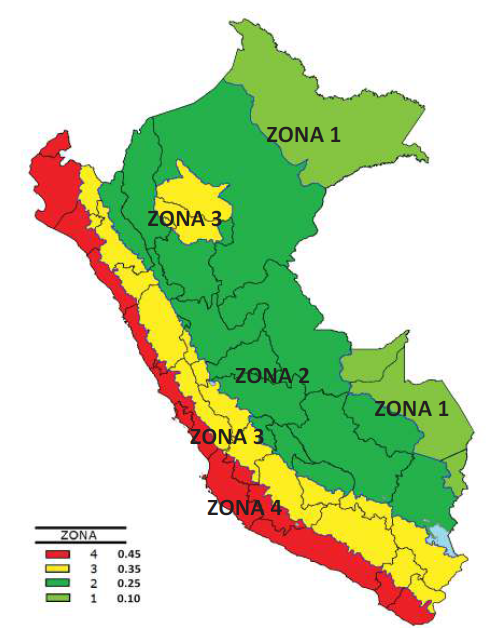
\includegraphics[width=4cm]{images/mapa_zona}%
\end{center}%
\end{minipage}%
\caption*{Fuente: E-30 (2018)}%
\end{table}

%
Las rigideces laterales pueden calcularse como la razon entre la fuerza cortante del entrepiso y el correspondiente desplazamiento relativo en el centro de masas, ambos evaluados para la misma condición de carga. \newline%
%
\end{document}